%\chapter*{Неделя 5}
\protect\thispagestyle{fancy}
\section{}
Рассмотрим сигнал $y(t)$, полученный путём фиксации на время, равное шагу дискретизации $\Delta t$, мгновенных значений исходного сигнала $x(t)$ с помощью ЦАП.

\begin{figure}[!h]
	\centering
	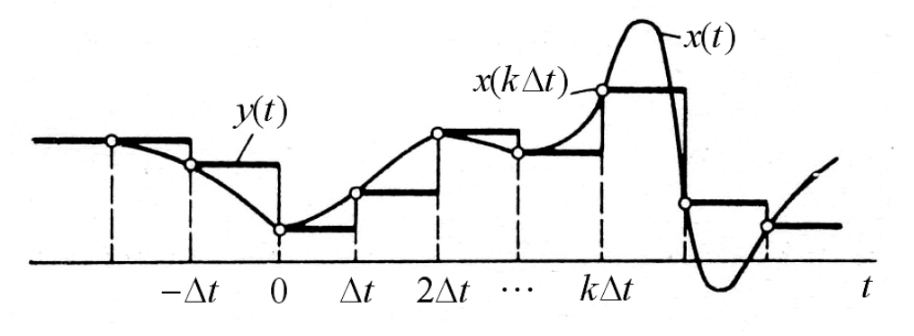
\includegraphics[width=0.5\columnwidth]{pics/fall/5/DAC.png}
	\label{fig:5-1}
\end{figure}

Пусть $x(t) = \sin(2\pi f_0 t)$, $-\infty < t < +\infty$ и шаг дискретизации $\Delta t = \frac{1}{10 f_0} = \frac{1}{f_d}$.

Определить частоты, амплитуды и фазы гармонических компонент на выходе фиксатора. Получить аналитическое выражения для выходного сигнала фиксатора как суперпозицию этих компонент.

Частотная характеристика интерполятора:
\begin{equation*}
	\Capit{H}(f) = \dfrac{\sin(\pi f \Delta t)}{\pi f} e^{-j \pi f \Delta t} = 
	\dfrac{\sin(\pi f/f_d)}{\pi f} e^{-j \pi f / f_d}.
\end{equation*}

Спектр дискретизованного сигнала на входе:
\begin{equation*}
	\Capit{X}_{d}(f) = \dfrac{1}{2j} \sum \limits_{m = -\infty}^{+\infty} 
	\big[\delta(f - f_0 + m f_d) - \delta(f + f_0 + m f_d)\big].
\end{equation*}

Спектр выходного сигнала (по теореме о свёртке):
\begin{equation*}
	\Capit{Y}(f) = \Capit{H}(f) \cdot \Capit{H}_{d}(f) = \dfrac{\sin(\pi f/f_d)}{\pi f} \dfrac{e^{-j \pi f / f_d}}{2 j} \sum \limits_{m = -\infty}^{+\infty} 
	\big[\delta(f - f_0 + m f_d) - \delta(f + f_0 + m f_d)\big].
\end{equation*}

Выходной сигнал:

\begin{align*}
	y(t)&=\int\limits_{-\infty}^{+\infty} \Delta t \dfrac{\sin (\pi f / f_{d})}{\pi f / f_{d}} \dfrac{e^{-j \pi f / f_{\mathrm{d}}}}{2 j} 
	\sum \limits_{m = -\infty}^{+\infty} 
	\big[\delta(f - f_0 + m f_d) - \delta(f + f_0 + m f_d)\big] e^{j 2 \pi f} d f=\\
	&=\sum_{m=-\infty}^{+\infty} \Delta t \left\{\dfrac{\sin \left(\pi\left(f_{0}+m f_{d}\right) / f_{d}\right)}{\pi\left(f_{0} + m f_{d}\right) / f_{d}}\right\}
	\sin \Big(2 \pi\left(f_{0}+m f_{d}\right) t -\pi\left(f_{0}+m f_{d}\right) / f_{d}\Big)=\\
	&=\sum_{m=-\infty}^{+\infty} \Delta t \left\{\dfrac{\sin \left(\pi\left(f_{0} +m f_{d}\right) / f_{d}\right)}{\pi\left(f_{d} + m f_{d}\right) / f_{d}}\right\}
	\sin \left(2 \pi \left(f_0 + m f_d\right) \left(t - \frac{1}{2} \Delta t\right)\right)=\\
	&=\sum_{m=-\infty}^{+\infty} \dfrac{1}{10 f_0} \left\{\dfrac{\sin \left(\pi\left(m + 0.1\right)\right)}{\pi\left(m + 0.1\right)}\right\}
	\sin \left(2 \pi f_0 \left(1 + 10m\right) \left(t - \frac{1}{20f_0}\right)\right).
\end{align*}

Выходной сигнал представляет собой суперпозицию гармоник:
\begin{itemize}
	\item с частотами $f_{m} = f_0 (1 + 10m)$,
	\item с амплитудами $\Capit{A}_m = \left|\dfrac{1}{10 f_0} \dfrac{\sin \left(\pi\left(m + 0.1\right)\right)}{\pi\left(m + 0.1\right)} \right|$,
	\item с фазами $\phi_m = -\pi (m + 0.1)$.
\end{itemize}



\section{}
Последовательность $x[k]$ из $1000$ элементов получена в результате дискретизации непрерывного сигнала $x(t)$ с частотой $f_d = 20480$ Hz. Обозначим через $\Capit{X}[n]$ $1024$-точечное ДПФ ($N = 1024$) последовательности $x[k]$ (дополненной нулевыми отсчётами). 
Определить расстояние (в Hz) между непрерывными частотами, которые соответствуют соседним отсчётам ДПФ.

Расстояние между соседними бинами ДПФ равно:
\begin{equation*}
	\Delta f  = \dfrac{1}{N} f_d = \dfrac{20480\text{ Hz}}{1024} = 20\text{ Hz.}
\end{equation*}

\section{}
Вещественный сигнал $x(t)$ с полосой $2f_b = 10$ KHz ($f_b$ -- верхняя граничная частота) дискретизуется с шагом $\Delta t$. В результате получается последовательность отсчётов $x[k]$. Вычисляется $N$-точечное ДПФ, где $N = 2^m$, $m \in \mathbb{N}$.

Определить минимальное значение $m$, при котором анализ возможен, а расстояние между отсчётами ДПФ по оси частот в герцах будет меньше $5$ Hz. Для этого значения $m$ определить допустимые пределы для частоты дискретизации $f_{\min} < f_d < f_{\max}$.

Чтобы разрешение по частоте оказалось меньше $\Delta f = 5$ Hz, необходимо:
\begin{align*}
	\Delta f > \dfrac{f_d}{N} = \dfrac{f_d}{2^m}\quad \Leftrightarrow \quad m > \log_2 \left( \frac{f_d}{\Delta f} \right).
\end{align*}

Чтобы анализ был возможен $f_d = f_{\min} = 2f_b = 10$ KHz, тогда $m = 11$.

Теперь для фиксированного $m$ найдём максимально возможную частоту дискретизации $f_d = f_{\max}$:
\begin{equation*}
	\Delta f > \dfrac{f_d}{N} = \dfrac{f_d}{2^m}\quad \Leftrightarrow \quad f_d < \Delta f \cdot 2^m  = 10240\text{ Hz.}
\end{equation*}

В итоге: $m = 11$, $f_{\min} = 10000$ Hz, $f_{\max} = 10240$ Hz.
